% Datos extraídos de doc/results/p2_baseline.json y p2_post.json
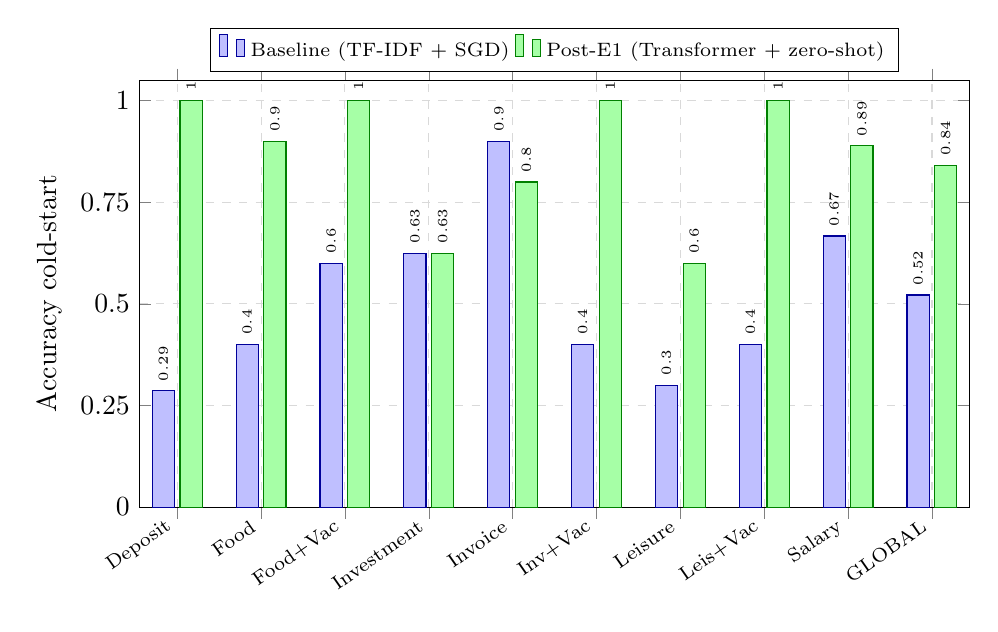
\begin{tikzpicture}
\begin{axis}[
    width=\linewidth, height=7cm,
    ybar=2pt,
    bar width=8pt,
    ylabel={Accuracy cold-start},
    ymin=0, ymax=1.05,
    ytick={0,0.25,0.5,0.75,1.0},
    yticklabel={\pgfmathprintnumber[fixed,precision=2]{\tick}},
    symbolic x coords={Deposit, Food, Food+Vac, Investment, Invoice, Inv+Vac, Leisure, Leis+Vac, Salary, GLOBAL},
    xtick=data,
    x tick label style={rotate=35,anchor=east,font=\scriptsize},
    legend style={at={(0.5,1.02)},anchor=south,legend columns=2,font=\scriptsize},
    nodes near coords,
    nodes near coords style={font=\tiny, rotate=90, anchor=west},
    every node near coord/.append style={/pgf/number format/.cd, fixed, precision=2},
    grid=major,
    grid style={dashed, gray!30},
    enlarge x limits=0.05,
]
\addplot[fill=blue!25,draw=blue!60!black] coordinates {
  (Deposit,0.286) (Food,0.400) (Food+Vac,0.600) (Investment,0.625)
  (Invoice,0.900) (Inv+Vac,0.400) (Leisure,0.300) (Leis+Vac,0.400)
  (Salary,0.667) (GLOBAL,0.522)
};
\addplot[fill=green!35,draw=green!50!black] coordinates {
  (Deposit,1.000) (Food,0.900) (Food+Vac,1.000) (Investment,0.625)
  (Invoice,0.800) (Inv+Vac,1.000) (Leisure,0.600) (Leis+Vac,1.000)
  (Salary,0.889) (GLOBAL,0.841)
};
\legend{Baseline (TF-IDF + SGD), Post-E1 (Transformer + zero-shot)}
\end{axis}
\end{tikzpicture}
